% !TEX encoding = UTF-8 Unicode
% !TEX program = pdflatex
% !TEX spellcheck = en_US


% In order to correctly compile this document,
% execute the following commands:
% 1. pdflatex
% 2. pdflatex
% 3. pdflatex



\documentclass[amsthm,ebook]{saparticle}

% IF YOU USE PDFLATEX
\usepackage[utf8x]{inputenc}
% if you write in english and in greek
\usepackage{ucs}
\usepackage[greek,english]{babel}
\languageattribute{greek}{polutoniko}

% IF YOU USE XELATEX
%\usepackage{polyglossia}
% if you write in italian
%\setmainlanguage{italian}
% If you want put some ancient greek:
%\setotherlanguage[variant=polytonic]{greek}
%\newfontfamily{\greekfont}[Ligatures=TeX]{Palatino Linotype}

% dummy text (remove in a normal thesis)
% remove if not necessary
\usepackage{siunitx}
%Natbib for bibliography management
\usepackage[authoryear]{natbib}
% custom commands
\newcommand{\bs}{\textbackslash}

%%%%%%%%
%TITLE:%
%%%%%%%%
\title{AUGMENTING THE WORKSPACE OF EPIGRAPHISTS
An interaction design study}

\author[1]{Angelos Barmpoutis\corref{first}}
\author[2]{Eleni Bozia}
\address[1]{Digital Worlds Institute, University of Florida}
\address[2]{Department of Classics, University of Florida}
\cortext[first]{Corresponding author. Email: angelos@digitalworlds.ufl.edu}
\date{2015-11-21}
\begin{document}

\maketitle
\begin{abstract}
This paper presents the results of an interaction design study that focuses on the use of natural user
interfaces for professionals in the fields of epigraphy and archaeology. This study proposes solutions for utilizing
the sensors that can be found in popular handheld devices, such as tablets and smart phones, in order to naturally
perform common tasks from the typical workflow of epigraphists. The developed interface allows the users to naturally
hold digitized inscriptions, interact with them in order to relight or manipulate them as if they were real physical
objects, and interact with metadata or other multi-modal data, such as text and images. 
\end{abstract}
\keywords{Mobile Applications, Interaction Design, Natural User Interfaces, 3D models, Archaeology}

\section{Introduction}


The technological advances in the last decade have equipped the general public with several handheld electronic
commodities that changed significantly daily routine in a personal and professional level and contributed to the user's
quality of life not only in developed countries but also in developing economies in Africa and Asia [Osman 2011].
Handheld devices, such as tablets and smart phones, not only connect the users with tremendous amount of information
through the internet, but also offer interfaces for natural user interaction that enable non-technology-oriented
populations to use computers intuitively.

In the fields of epigraphy and archaeology, the areas of digital epigraphy and computational archaeology have benefit
from the use of several of the sensors available in hand-held devices. Crowd-sourcing of photographic data and
geo-spatial information, augmented-reality navigation in archaeological spaces and museums, and 3D scanning of
historical artifacts, using smart phones and tablet computers,, are few of the exemplar applications of hand-held
sensors in epigraphy and archaeology. One common component in all the aforementioned applications is the ability to
record tridimensional data either in the form of geo-spatial coordinates, or in the form of local 3D point coordinates
needed for augmented-reality interaction, or for the construction of triangular meshes of 3D models. 

There are several examples in literature that present 3D digitization projects that have been undertaken by museums
including the Epigraphical Museum of Athens (\citet{sullivan_analytical_2011}, \citet{papadaki_accurate_2015}), Museo Arqueológico Nacional de
Madrid \citep{ramirez-sanchez_epigrafidigital:_2014}, Museo Nazionale Romano di Palazzo Altemps \citep{barmpoutis_interactive_2015}, Museo
Geologico Giovanni Capellini di Bologna \citep{abate_valorizzazione_2014}, National Museums Liverpool \citep{cooper_chiswick_2007},
Smithsonian Institution \citep{wachowiak_3d_2009}, and several other museums and institutes (\citet{barsanti_3d_2013}, \citet{landon_petroglyph_2006}, \citet{levoy_digital_2000}).

Several novel methods for scanning, processing, and analyzing 3D models of inscriptions have been developed, including
methods for text extraction from inscriptions (\citet{aswatha_method_2014}, \citet{sullivan_analytical_2011}), accurate 3D scanning of
inscriptions \citep{papadaki_accurate_2015}, visualization of inscriptions \citep{bozia_open-access_2014}, as well as 3D applications for
other archaeological artifacts (\citet{babeu__2011}, \citet{pollefeys_image-based_2001}, \citet{malzbender_polynomial_2001}, \citet{esteban_silhouette_2004}).
Comparative studies of 3D scanning methods for cultural herirage can be found in \citep{pavlidis_methods_2007} and \citep{bohler_3d_2004}. 

The aforementioned examples show that the use of 3D technologies in epigraphy and archaeology has been a
well-studied topic over the past two decades. However, there is a notable disconnect between the research on these
technologies and the actual use in the professional epigraphic and archaeological practice as it has been hard for
non-technology-oriented audiences to handle and manipulate tridimensional data, using conventional computer equipment.
Furthermore, without mechanisms for proper user interaction, a 3D model that is projected on a 2D screen is not
significantly advantageous compared to a set of 2D photographs. 

The recent advances on Natural User Interfaces (NUI) along with their marketing as low-cost general-purpose devices
(smart phones and tablets) have created a nurturing environment for integrating them in cultural heritage applications.
Popular low-cost NUIs, such as touch screens, marker-less position trackers, motion sensors, and head-mounted displays
have been recently studied and employed by museums as mechanisms for multi-sensory virtual experiences (\citet{ujitoko_application_2015}, \citet{soile_accurate_2013}, \citet{ikei_experience_2015}).

This paper tries to fill the gap between the 3D technologies and their actual professional application in the field of
epigraphy by proposing innovative uses of NUIs specially designed to serve epigraphists. This is, to the best of our
knowledge, the first systematic interaction design study in the field of epigraphy. This study proposes solutions for
utilizing the sensors that can be found in popular handheld devices to naturally perform common tasks from the typical
workflow of epigraphists. The developed interface allows the users to naturally hold digitized inscriptions and
interact with them in order to relight or manipulate them, as if they were real physical objects, and also interact
with metadata or multi-modal data, such as text and images. 

\section{Understanding the workflow of epigraphists}


Understanding the users is one of the integral steps of interaction design, which is an iterative process during which
representative users interact with preliminary designs and provide useful feedback \citep{preece_interaction_2015}. For the
purposes of this study, our team interacted with early adopters of our prototype system, who were epigraphists and
conservation specialists from Cornell University, the University of California, Berkeley, the University of Lyon 2, the
Berlin-Bradenburg Academy of Sciences and Humanities, the U.K. National Archives, and the University of Florida. The
goals of our interaction were twofold: a) to study the various forms of physical interaction that epigraphists have
with an inscription as a real physical object and b) to expose epigraphists to a digital interface that imitates
their interaction routine, using digital replicas of physical objects.

The first part of our study revealed 3 common types of interaction with the inscriptions as physical objects:

\begin{enumerate}
\item Change of point of view: Observation of the inscription from different viewing angles assists epigraphists
understand better the shape of the inscribed letterforms. 
\item Change of lighting conditions: Relighting the inscription by introducing artificial shadows or additional light
sources from different angles may reveal details that were not legible in the original lighting conditions.
\item Magnification of inscribed details: Close observation of an inscribed region of interest, with or without
artificial magnification, may assist epigraphists in assessing weathered fragments and make a better informed decision
regarding the deciphering of the original text.
\end{enumerate}
It should be noted that in addition to the above 3 types of interaction, there are two additional interactions that are
special cases of I and II. More specifically, the physical object can be either portable (such as a small fragment of
stone or other material) or not (when the inscription is on an inscription bearer). In the case of a handheld object,
interactions I and II involve manual movement of the inscription with respect to the fixed observer (case I) or the
fixed light source (case II), while in the case of large rigid objects the observer and the light source move with
respect to the fixed inscription. 

According to the above analysis, in the case of digitized inscriptions a NUI should provide the means for an epigraphist
to ``hold'' the virtual object, ``move'' the point of view with
respect to the virtual object, ``manipulate'' the virtual object with respect to the virtual
light source, and ``focus'' on details of interest. The next section presents a NUI-based
interaction design that proposes natural solutions to the aforementioned forms of interaction that seamlessly imitate
the typical workflow of epigraphists. 

\section{Natural User Interface design for epigraphy}


Natural User Interfaces consist of sensors that track the natural behavior of users and provide a natural form of
interactivity with computers and other electronic devices. The common forms of NUI sensors are: pressure sensors for
sensing touch gestures (e.g. touch screens and touch pads), motion sensors for sensing user-initiated changes in the
orientation and acceleration of the device (e.g. accelerometer, gyroscope, and compass), and position sensors for
tracking changes in the relative position of the user with respect to the device, such as body motions (e.g.
Microsoft's Kinect), finger motions (e.g. Occipital's Leap Motion), eye movements, and others.

\ An optimal interaction design solution should be intuitive, minimalistic, and non intrusive \citep{preece_interaction_2015}.
Therefore, in order to design interaction for epigraphy one should choose devices that are easily accessible by
epigraphists and do not interfere with their workspace (e.g. avoid introducing new devices or external sensors). All
forms of interaction described in Sec. 1.2 can be implemented, using motion and pressure sensors, which can be easily
found in tablet computers or smart phones. In both types of handheld devices the virtual object can also be assumed
handheld, without loss of generality, in order to generate a multi-sensory experience for the user (i.e. holding the
device = holding the digital inscription). Hence, NUI design is possible by utilizing accessible devices and
without the use of external sensors as it is described in details in the following sections.


\subsection{Natural interactive relighting of 3D models}


In order to achieve natural interactive relighting of an inscription, the system should imitate the process of
relighting a handheld physical object (such as a paper cast of inscription) by reorienting the object with respect to
the light of the environment. Without loss of generality, we can assume that the default virtual lighting source is
located on the ceiling, right above the device, which is also very intuitive choice as it is the most probable
real-world lighting condition. Under this assumption, a gyroscope, a sensor that tracks the orientation of the device
with respect to the gravitational vector, is enough to track the slope of the device with respect to the virtual light.
The top row of Fig.~\ref{fig:1} shows the approximated real-world orientation of a tablet computer as it was estimated using
the gyroscope of the device. The orientation is updated in real-time as the user moves the device.

\begin{figure}[!bp]
\centering
 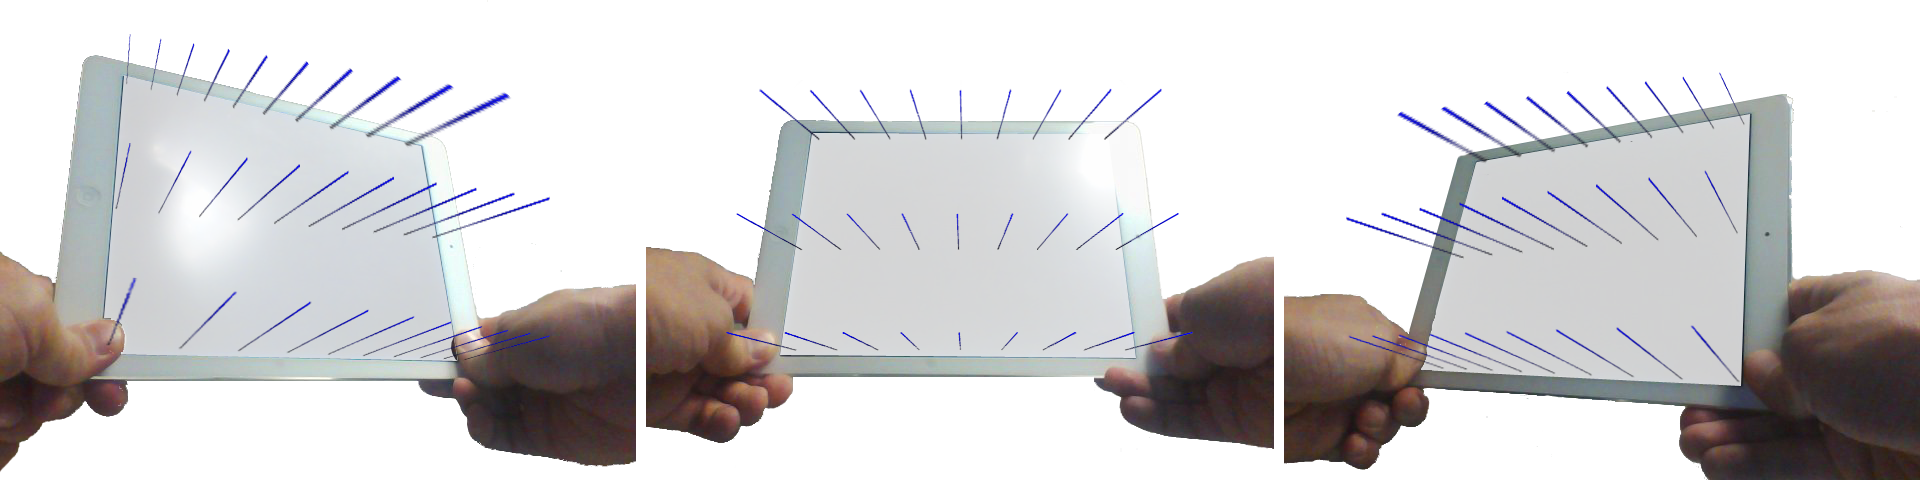
\includegraphics[width=\columnwidth]{EAGLE2016cameraready-img001.png}
 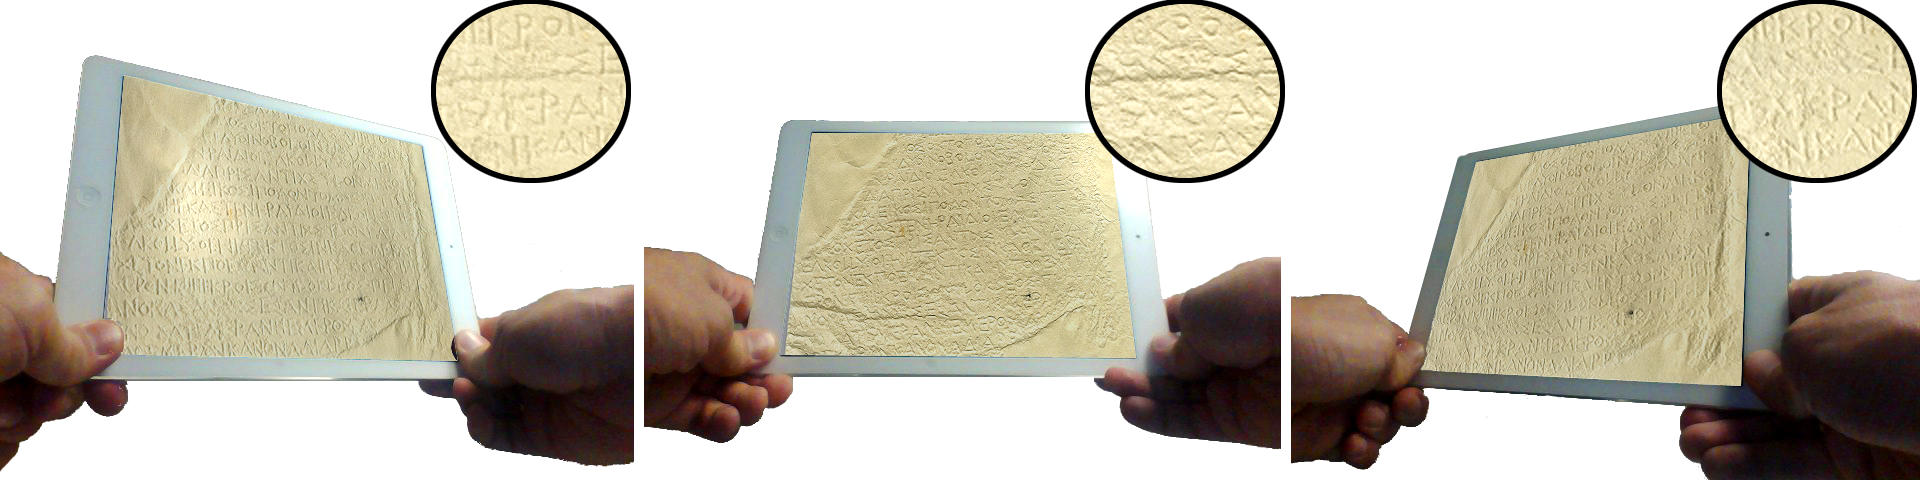
\includegraphics[width=\columnwidth]{EAGLE2016cameraready-img002.png}
\caption{ Top row: Illustration of interactive manipulation of the virtual lighting by moving the device. The figures
show the corresponding field of normal vectors in the 3D space as computed using the gyroscope of the device. Bottom
row: Demonstration of interactive relighting of a 3D digitized inscription. Different virtual lighting angles reveal
different inscribed details. }
\label{fig:1}
\end{figure}

 

The estimated orientation of the device can be used in order to relight the depicted 3D model of inscription using the
angle of the device with the direction of the virtual light source. The bottom row of Fig.~\ref{fig:1} demonstrates interactive
relighting of a digitized paper cast. Epigraphists can relight an inscription by reorienting the tablet as if it were a
real physical object. This process matches perfectly with the physical interaction of epigraphists with real
inscriptions and can be intuitively extrapolated to the case of 3D models of large inscriptions that were not handheld
in the real world (see Fig.~\ref{fig:3}).




\subsection{Natural interactive manipulation of 3D models }


Another important form of interaction in the epigraphic routine is the change of the point of view in order to
understand better the structural details of the inscribed letterforms. Assuming that the model of the inscription is
parallel to the screen of the device, the change of point of view involves only change of the perspective projection of
the digital object without any virtual rotation. In such case the rotation of the object is equivalent to the physical
rotation of the device without any virtual rotation of the object.

Fig.~\ref{fig:2} shows 15 different projections of the same virtual cube that correspond to the change of perspective caused
by moving the observer's head parallel to the screen. Note that all cubes are parallel to each other.




\begin{figure}[!bp]
\centering
 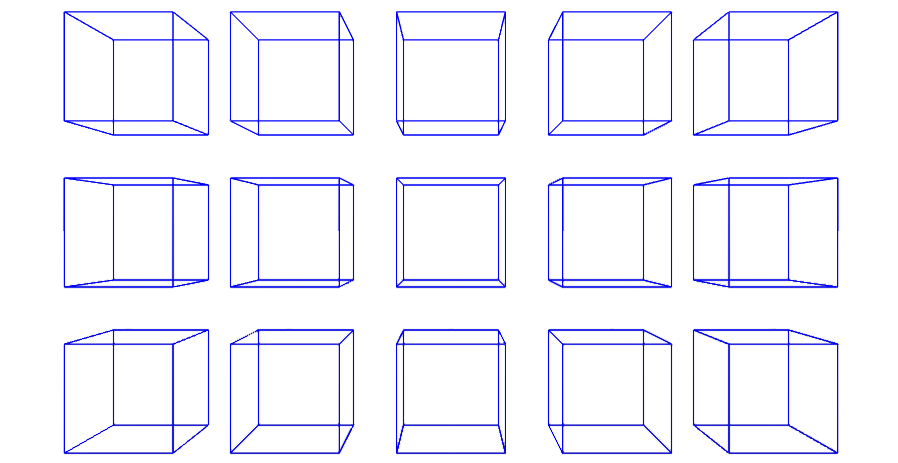
\includegraphics[width=\columnwidth]{EAGLE2016cameraready-img003.png}
\caption{Visualization of same-size boxes using 15 different perspective projections with the same FOV angle and
different cropping parameters. None of the boxes is rotated in the space. }
\label{fig:2}
\end{figure}





In the case of a tablet computer, the change of perspective can be implemented using the accelerometer of the device,
which senses non-gravitational accelerations in the 3D space. With the logical assumptions that: a) the tablet is
initially facing the user, and b) the user's eyes remain in a relatively fixed position in the 3D space (otherwise an
eye-tracker should be required), the change of perspective can be realistically achieved by naturally reorienting the
tablet as shown in the top row of Fig.~\ref{fig:3}. The superimposed boxes in this figure were estimated, using the
accelerometer reading of the device for three different orientations of the tablet. 

Interactive manipulation of a 3D digitized inscription bearer is shown in the bottom row of Fig.~\ref{fig:3}. Different sides of
the bearer can be observed by reorienting the tablet naturally. In this example a large inscription model with its
bearer was chosen in order to demonstrate that the proposed interaction design remains intuitive independently of the
scale. It should also be noted that the interactive manipulation of the perspective can be optionally performed
simultaneously with the interactive relighting as shown in Fig.~\ref{fig:1} (bottom) in order to perform a more realistic
interaction that causes relighting and change of point of view at the same time. 




\begin{figure}[!bp]
\centering
 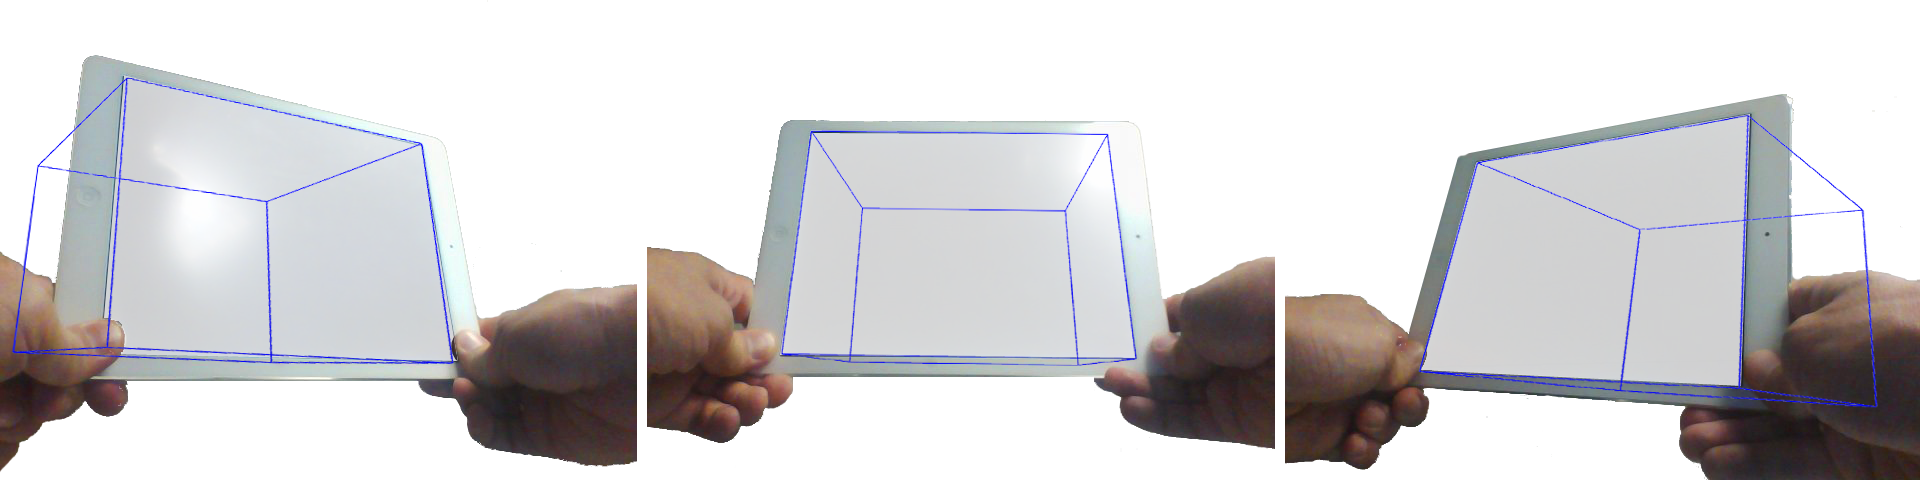
\includegraphics[width=\columnwidth]{EAGLE2016cameraready-img004.png}
 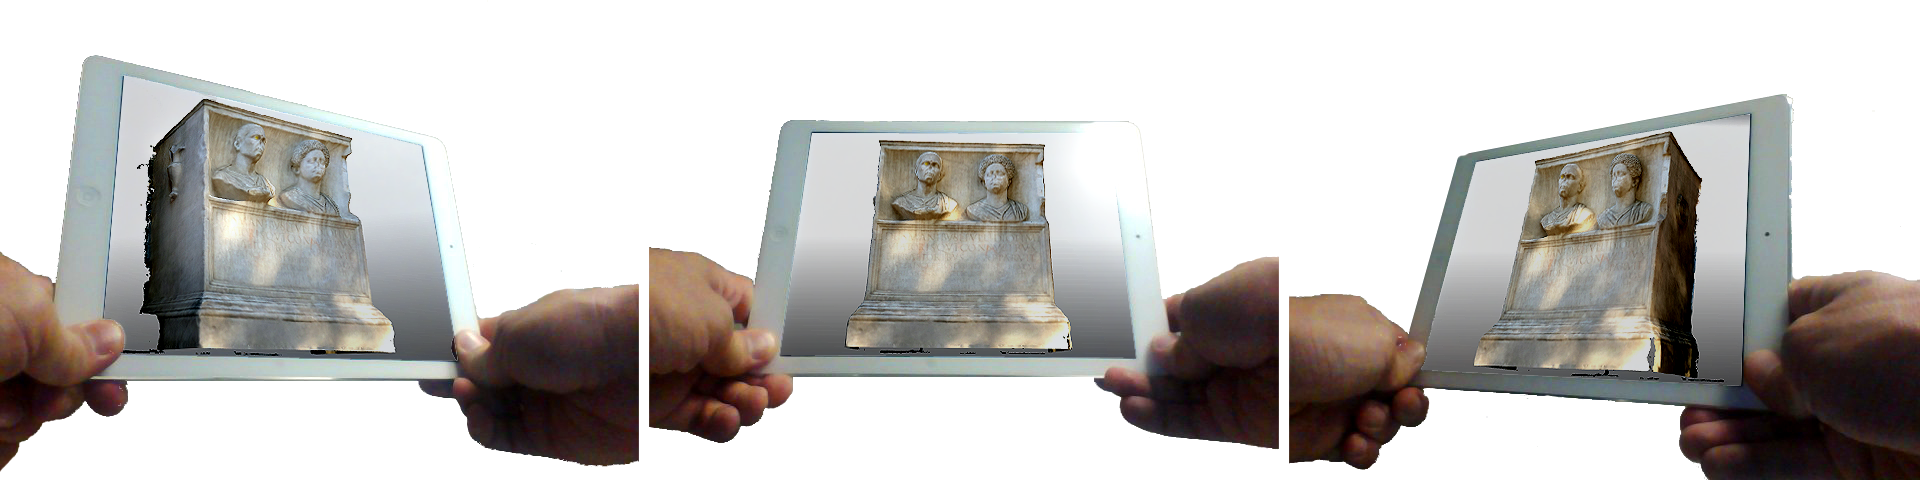
\includegraphics[width=\columnwidth]{EAGLE2016cameraready-img005.png}
\caption{Top row: Illustration of interactive manipulation of the perspective projection by moving the device and using
the {\textquotedbl}fixed eye{\textquotedbl} assumption. Bottom row: Demonstration of interactive visual inspection of a
3D digitized inscription along with the inscription bearer. The user can view the object from different perspectives,
using natural motions.}
\label{fig:3}
\end{figure}



\subsection{``Touching'' the metadata: Interacting with multi-modal data}


The forms of interactions presented in 1.3.1 and 1.3.2 involved only the motion sensors of a tabled computer without
utilizing the pressure sensors of the screen of the device. The commonly used touch gestures (such as 2-finger twist to
rotate, 2-finger pinch to zoom, and 2-finger translate to move) can be employed in order to enhance the proposed NUI
design. In addition to the aforementioned gestures, a tap gesture could activate regions of interest with additional
modalities of information such as text, images, and metadata. The user can interactively browse the different forms of
data by using intuitive touch gestures as shown in Fig.~\ref{fig:4}. This set of 2D interactions along with the 3D NUI design
presented earlier can compose an intuitive yet powerful workspace for an epigraphist who can now perform digitally
several parts of the epigraphic workflow. 




\begin{figure}[!bp]
\centering
 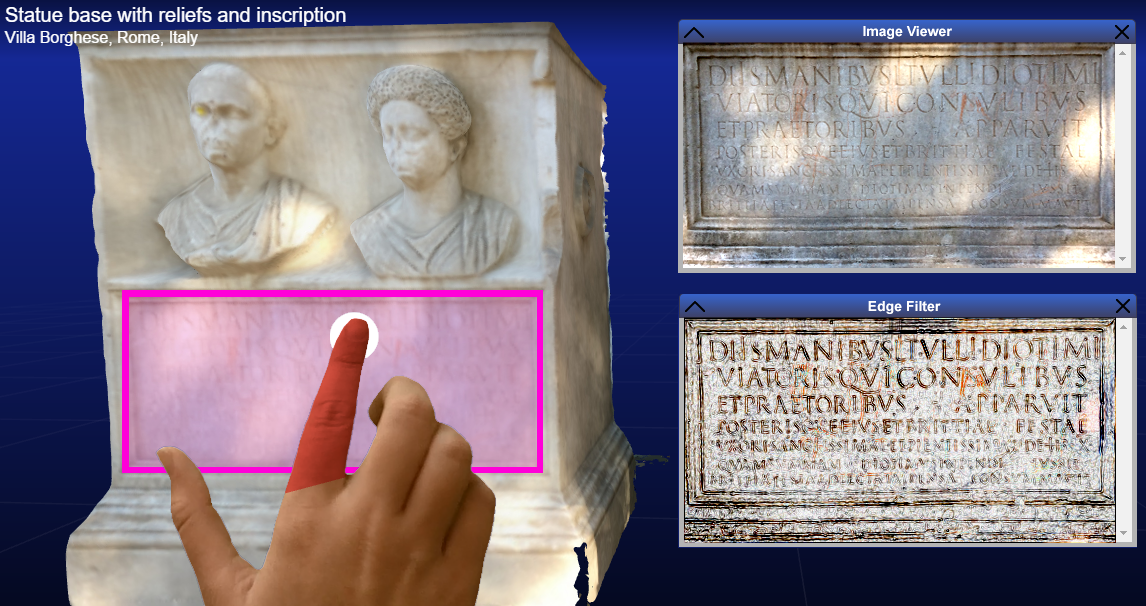
\includegraphics[width=\columnwidth]{EAGLE2016cameraready-img006.png}
\caption{Screenshot of our interactive environment. The user interacts with the 3D object, using touch gestures and
selects one of the regions of interests. This action initiates other data tools such as the image viewer or the edge
filter as shown in this example}
\label{fig:4}
\end{figure}

\section{Conclusions and future directions}


In this pilot study, a complete set of natural user interactions was designed based on the physical interactions of
epigraphists with real inscriptions. The proposed interactions utilize the existing sensors in a typical tablet
computer or smart phone in order to interactively relight a digitized inscription and manipulate the user's
perspective, using a set of intuitive gestures that imitate the natural interaction with a physical object. In the
proposed design, the epigraphist can ``hold'' a digital inscription, relight it by
reorienting it as a tangible object, observe it from different perspectives, and finally interact with other modalities
by following a set of 2D touch gestures. The prototype system was developed as part of the Digital Epigraphy and
Archaeology (DEA) project using the open-source library VisiNeat for 3D visualization and interaction and is compatible
with iOS, Android, and Microsoft RT tablet and smart phone devices. The interface is available through the web-site of
the project: http://www.digitalepigraphy.org

In the future we plan to quantitatively evaluate the designed interface by tracking the user activities and analyze
their motion patterns in the 3D space while they are interacting with their handheld device. 



\section*{Acknowledgement}

We would like to acknowledge our collaborators for their invaluable interaction and feedback during the past three
years. We would also like to thank the UF College of the Arts and the UF Center for Greek Studies for providing
continuous funding support for this project. 

\bibliographystyle{sapauth-eng}
\bibliography{../../EAGLE}

\end{document}
